% !TEX root = catron-dissertation.tex
\epstopdfsetup{outdir=./images/06_single_sensor_filtering/}

\chapter{Wavefront Multidimensional Spectral Filtering Techniques}
\label{chap:06_single_filter}
% \textcolor{red}{
%   \begin{itemize}
%     \item Work on the chapter intro
%     \item Filter applied in Fourier space and multidimensional spectral space
%   \end{itemize}
% }

This chapter will examine a variety of filtering techniques used on multidimensional spectra of optical wavefronts.
While none of the filters presented here are novel, many are based on well known digital filters, their application to filtering optical wavefronts is something that needs to be studied.

By Using multidimensional spectral estimates on wavefronts, as shown in Chapter \ref{chap:04_dispersion}, differences in source disturbances become clearly evident.
When just the wavefront measurement itself is available, digital filters can be used to separate or isolate a single disturbance source or at least minimize the impact from other sources.
The digital filters used in this dissertation, use a transfer function, $H(j\omega)$, and are applied in Fourier space.
The transfer functions themselves are typically derived in Laplace space, $H(s)$, but because $s=j\omega$ they are valid in Fourier space as well \cite{Hamming-1998-CdhcDuvZ}.
The transfer function is compromised of two components which attenuate the signal, gain and phase.
The filter gain is the magnitude of the transfer function, $G(\omega) = |H(j\omega)|$, while the filter phase is the argument, $\Phi(\omega) = \arg(H(j\omega))$.
In the simplest case, the filtered signal is the inverse Fourier transform of the gain multiplied by the Fourier transform of the signal,
\begin{equation}
 f_F(\mathbf{x}) = \real\left(\ifftn[H(j\mathbf{\omega})\fftn\{\mathbf{x}\}]\right) \textrm{,}
 \label{eqn:06_filter_function}
\end{equation}
where $f$ is the signal function and $f_F$ is the filtered signal.

\section{Temporal Filter Methods}
The methods presented in this section are based on Butterworth filters but could be extended to other types of filters.
The square of the transfer function of a Butterworth filter is \cite{Butterworth-1930-DvDrjKha},
\begin{equation}
 |H(j\omega)|^2 = G^2(\omega) = \frac{G_0^2}{1+\left(\frac{j\omega}{j\omega_c}\right)^{\pm2n}} \textrm{,}
 \label{eqn:06_butterworth}
\end{equation}
where $G_0$ is the zero-frequency gain, $\omega_c$ is the cutoff angular frequency, $n$ is the filter order (number of filters in a series), and $\pm$ represents either a low-pass ($+$) or high-pass ($-$) filter.
The gain of this filter is
\begin{equation}
  G(\omega) = \frac{G_0}{\sqrt{1+\left(\frac{\omega}{\omega_c}\right)^{\pm2n}}} \textrm{.}
  \label{eqn:06_butterworth_gain}
\end{equation}
A band-pass filter can be constructed by placing a low-pass filter in series with a high-pass filter and a band-stop by placing the two types in parallel.

In many tests, a large portion of the wavefront noise is at low frequencies primarily caused by mechanical vibration.
In general, a high-pass filter is useful in temporal space for removing this noise, since in many cases most of the power in the aero-optical signal occurs at higher frequency than the low-frequency mechanical vibration. as shown in Figure \ref{fig:06_filter_temporal}.
\begin{figure}
 \centering
 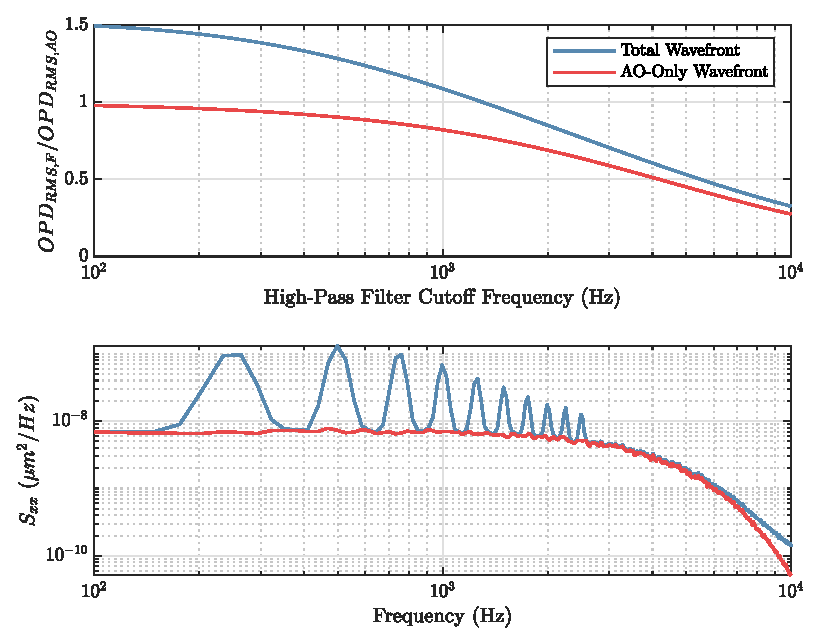
\includegraphics{../matlab/06_single_sensor_filtering/filter_temporal.eps}
 \caption{The $opdrms$ of high-pass temporal filtered wavefronts relative to the $opdrms$ of the aero-optical only unfiltered wavefront (top). Power spectra of both of the simulated wavefront versions (bottom).}
 \label{fig:06_filter_temporal}
\end{figure}
The top plot in this figure shows the high-pass filtered $\opdrms$ of both the total and aero-optical only wavefronts normalized by the unfiltered $\opdrms$ of the aero-optical only wavefront, for high-pass filters with various cutoff frequencies.
The results in Figure \ref{fig:06_filter_temporal} were computed using wavefronts that were simulated using the methods described in Chapter \ref{chap:05_synthetic}.
For reference, the bottom plot of Figure \ref{fig:06_filter_temporal} shows the power spectra of just the aero-optical portion of the wavefront (red curve) and the total wavefront (blue curve) which includes vibration-related peaks associated with the blade-passing frequency and its harmonics.
The figure shows how a high-pass filter decreases the energy in the total wavefront and in the actual aero-optical wavefront, as the filter cutoff frequency increases.
As shown in the top plot, at low cutoff frequency, the filter primarily removes vibration effects from the total signal; however, as the cutoff frequency increases, the filter also removes actual aero-optical signal.
At around 1200 Hz, the $\opdrms$ of the total signal is equal to the $\opdrms$ of the actual aero-optical signal; at this cutoff frequency ~75\% of the aero-optical signal remains and the remaining signal is made up by the remaining contamination.
This approach can provide a computationally inexpensive way of estimating the aero-optical portion of the wavefront for calculations that rely on the $\opdrms$ of a wavefront.
While it is more straightforward to determine a cutoff frequency for this synthetic wavefront since all of the signal components are fully known, a measured wavefront will likely take some knowledge or expectation of the contamination that is present in the measurement in order to select a high-pass filter cutoff frequency.

% \ref{tab:test}
% \begin{table}
% \centering
% \caption{Test Table}
% \input{../matlab/04_basic_filtering/filter_temporal.txt}
% \label{tab:test}
% \end{table}

An example of wavefronts that result from band-pass and band-stop filtering is shown in Figure \ref{fig:06_filter_temporal_bandpass}.
\begin{figure}
 \centering
 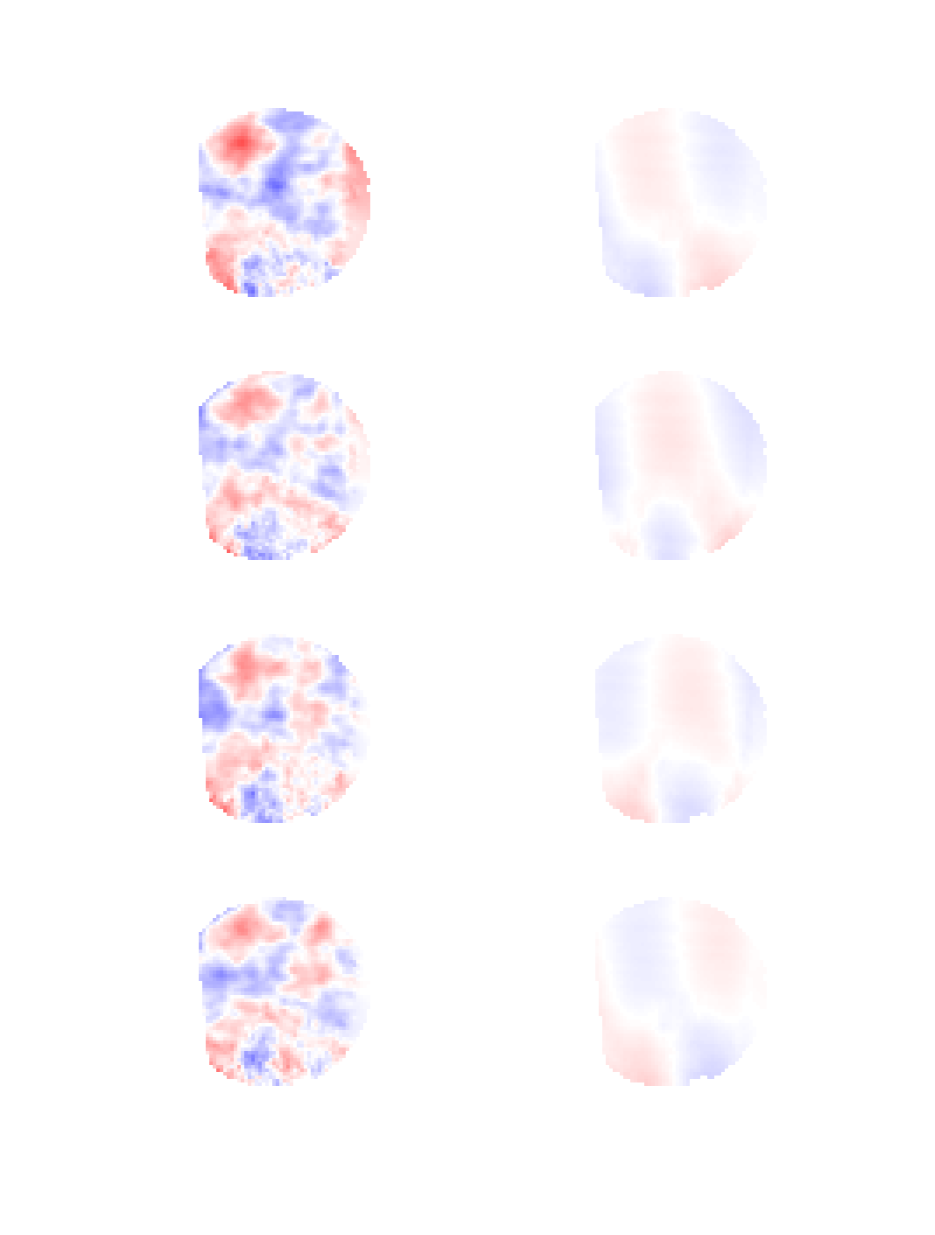
\includegraphics{../matlab/06_single_sensor_filtering/filter_temporal_bandpass.eps}
 \caption{Measured wavefronts filtered at the blade-passing frequency (532$\pm$10 Hz).  The left column is band-stop filtered while the right is band-pass filtered.}
 \label{fig:06_filter_temporal_bandpass}
\end{figure}
The figure shows several wavefront frames of measured data acquired in the Notre Dame White Field wind tunnel and presented previously in Chapter \ref{chap:03_optical_acoustics} (see Figure \ref{fig:03_tunnel_comparison}) that is band-stop filtered in the left column and band-pass filtered in the right column.
The flow is from right-to-left and the band-pass filtered wavefront clearly shows upstream-moving optical disturbances (moving left-to-right against the flow direction) associated with acoustic duct modes traveling upstream from the fan.
On the other hand, the band-stop filtered wavefronts on the left of Figure \ref{fig:06_filter_temporal_bandpass} show much slower-moving optical disturbances that are in general moving in the direction of the flow.
In particular, the downstream-moving disturbances on the left side of Figure \ref{fig:06_filter_temporal_bandpass} have the appearance of boundary-layer aero-optical disturbances, with a scale on the order of the boundary-layer thickness.

Note that for filters that operate in one dimension, the filters were applied over both positive and negative frequencies to of the n-dimensional Fourier transform in order to preserve the direction of travel of the signal.
This also allowed several filters to be applied in series with one another without having to perform a Fourier and inverse Fourier transform for each successive filter.
Temporal filters are also used in sizing and/or designing adaptive optics systems \cite{Greenwood-1977-aWDqUh6C} for example.
A low-pass filter with a cutoff at the bandwidth of either a fast-steering or deformable mirror is often used to define the signal that the system needs to reject \cite{Whiteley-2007-bHbWRWUu}.
A control system may need to have the bandwidth reduced in order to keep a mirror’s travel within limits \cite{Madec-2012-YJ8eWhPB}, while a high-pass filter would inform designers of the remaining optical aberrations that cannot be corrected.

\section{Upstream/Downstream Moving}
\label{chap:06_up_down_filter}
In the preceding section, filters based on temporal frequency only were discussed. In this section, another filtering approach is presented in which signals are identified based on their dispersion velocity.
For the filtering of upstream and downstream moving optical disturbances a logistic function was chosen,
\begin{equation}
 f(x) = \frac{1}{1+\exp\{-kx\}} \textrm{.}
 \label{eqn:06_logistic}
\end{equation}
This function was then expanded into two-dimensions ($x$ and $t$).
For a filter that removes disturbances moving against the direction of flow, the filter should ideally return a value of one in both the first and third quadrants and zero otherwise when plotted in a graph of temporal versus spatial frequency.
To accomplish this, the logistic curve in each dimension was scaled and offset to output values between negative one and positive one,
\begin{equation}
 G_t(f) = \frac{2}{1+\exp\{-k_tf\}}-1
 \label{eqn:06_logistic_time}
\end{equation}
and
\begin{equation}
 G_x(\xi_x) = \frac{2}{1+\exp\{\pm k_x\xi_x\}}-1 \textrm{,}
 \label{eqn:06_logistic_space}
\end{equation}
where $\pm$ determines whether the filter is designed to act on upstream-traveling disturbances ($+$) or downstream-traveling ($-$).
These two gain functions are then multiplied together and scaled to output values between zero and one,
\begin{equation}
 G(\xi_x,f) = \frac{(G_t\cdot G_x)+1}{2} \textrm{.}
 \label{eqn:06_up_down_filter}
\end{equation}
As the values of $k_x$ and $k_t$ go to infinity an ideal filter is obtained.
In a plot of the gain with the horizontal spatial frequency on the x-axis and the temporal frequency on the y-axis, an ideal filter for obtaining only the downstream traveling disturbances would have a gain of one in the first and third quadrants, zero in the second and fourth quadrants, and a value of $1/2$ when either frequency is zero.
The value of $1/2$ would equally split the component of a disturbance that is neither traveling upstream or downstream between the two directions.

The multidimensional spectrum using an ideal upstream-moving moving filter on the synthetic wavefront is shown in Figure \ref{fig:06_filter_downstream} alongside the spectrum of the unfiltered wavefront.
\begin{figure}
 \centering
 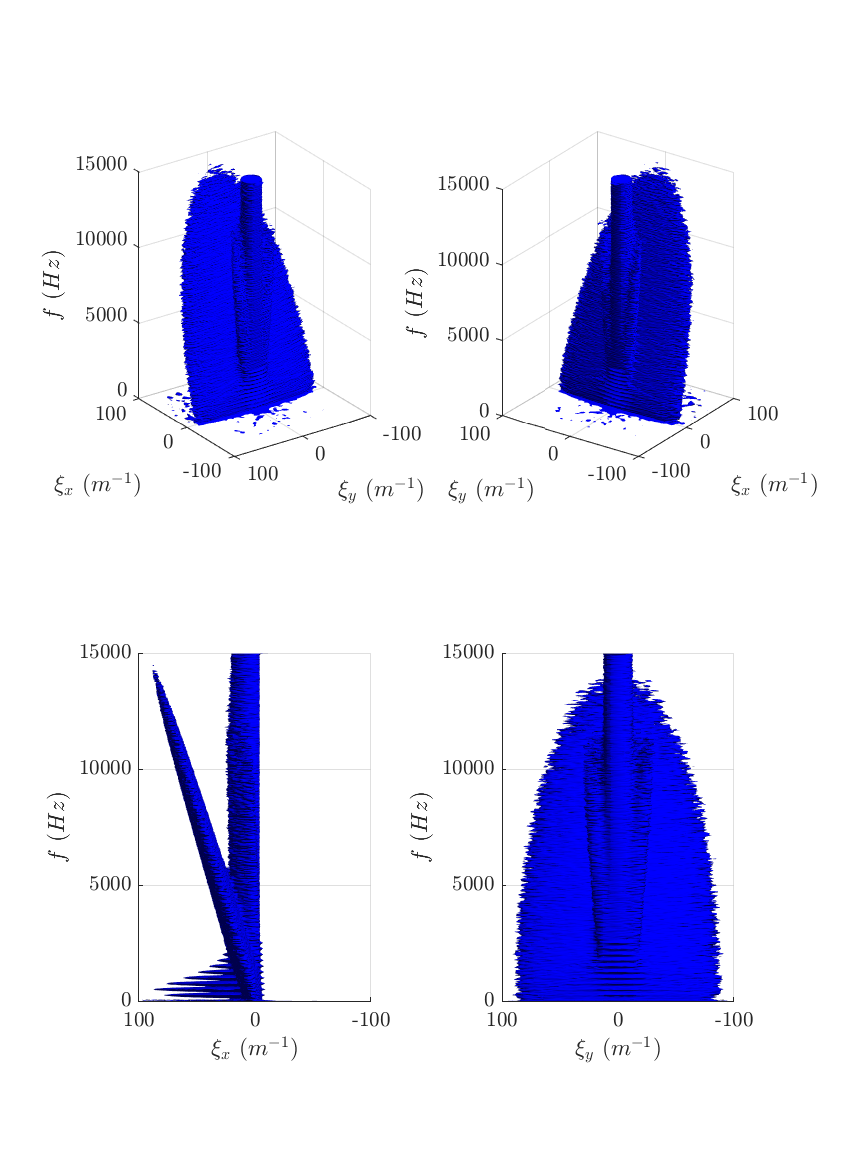
\includegraphics{../matlab/06_single_sensor_filtering/filter_downstream.eps}
 \caption{Multidimensional spectral isosurface of the synthetic wavefront with a downstream filter in place.}
 \label{fig:06_filter_downstream}
\end{figure}
All of the upstream traveling disturbances are removed and the disturbances at the stream-wise spatial frequency $\xi_x=0$ m$^{-1}$ are significantly reduced.
Some of the stationary modes (the vertical cylinder along $\xi_x=0$ and $\xi_y=0$) remain while only the acoustic and vibration signals that are propagating in the direction of flow remain.
The aero-optical signal from the boundary layer is clipped slightly at $\xi_x=0$ due to the spatial width of the signal.
The ratio of the time-averaged spatial-RMS of the filtered signal when compared to the aero-optical only signal was 1.24 while the unfiltered ratio was 1.53.
When the filter was applied to the wavefront with only the aero-optical boundary layer signal present the $\opdrms$ was reduced to 96\% that of the unfiltered wavefront.
This filter method will retain any disturbance that is traveling in the direction of flow.
Even with an ideal filter there is some slight attenuation of the aero-optical signal due to signal having some spectral width that crosses into upstream-moving portion of the dispersion plot.


\section{Velocity Filtering}
\label{chap:06_velocity_filter}
For a nondispersive medium such as air, flow structures traveling at a given speed have a constant slop on a multidimensional spectral plot.
A plane in the multidimensional spectral plot can therefore be used to measure a flow structure's velocity in both $x$ and $y$-directions.
The distance from any given point in the multidimensional spectral space to a plane described by the velocities $u_x$ and $u_y$ can be computed by
\begin{equation}
 d = \frac{|u_x\xi_x+u_y\xi_y-f|}{\sqrt{u_x^2+u_y^2+1}} \textrm{.}
 \label{eqn:06_dist_point_2_plane}
\end{equation}
Equation \ref{eqn:06_dist_point_2_plane} above can therefore be used to construct a low-pass or high-pass filter that retains only disturbances that are traveling at that velocity, or to exclude those disturbances,
\begin{equation}
  G(d) = \frac{1}{\sqrt{1+\left(\frac{d}{d_c}\right)^{\pm2n}}} \textrm{.}
  \label{eqn:06_butterworth_velocity}
\end{equation}
where $d_c$ is the cutoff distance from the plane defined by the velocities $u_x$ and $u_y$.
Because of difference in the temporal and spatial sample rates of several orders of magnitude, the filter function employed in this research used frequencies that have been normalized by the sample rate.

An example of a low-pass velocity-filter applied to the synthetic wavefront generated in Chapter \ref{chap:05_synthetic} is shown in Figure \ref{fig:06_filter_velocity}.
\begin{figure}
 \centering
 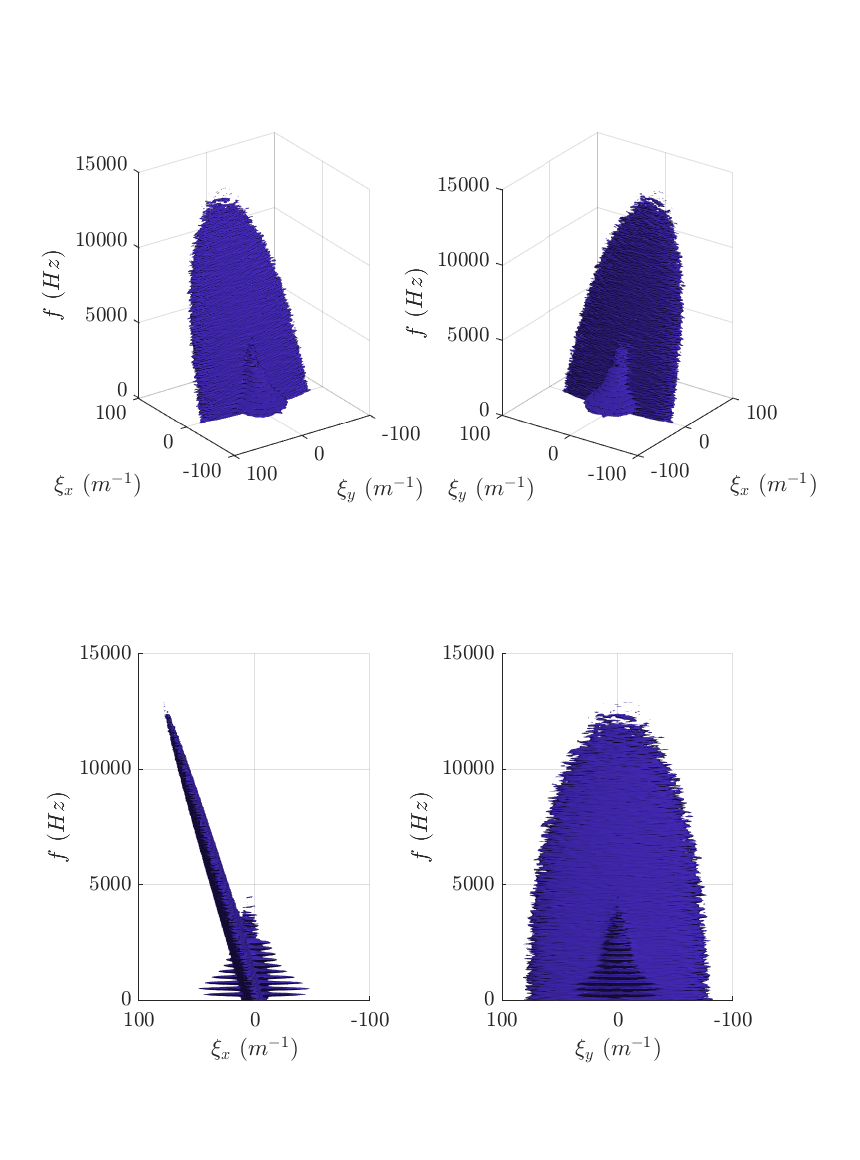
\includegraphics{../matlab/06_single_sensor_filtering/filter_velocity.eps}
 \caption{Multidimensional spectral isosurface of the synthetic wavefront with a low-pass velocity-filter in place.}
 \label{fig:06_filter_velocity}
\end{figure}
The filter was constructed for a $u_x$ set at the mean boundary-layer velocity and, $u_y$ set to zero.
The values of the other two filter parameters were selected as $d_c=1/80$, and $n=1$, which were chosen in a trial-and-error process in which values were chosen, the filtered multidimensional spectrum was computed, and refinements to the parameter values were made based on how well the filtered spectrum captured just the boundary-layer signal.
Figure \ref{fig:06_filter_velocity} shows that, using these filter parameters, the  velocity-filtered multidimensional spectrum successfully retains primarily only the aero-optical signal with some additional low-frequency content from the blade-passing frequency and harmonic disturbances as well as some stationary and acoustic disturbances.
The ratio of the $\opdrms$ relative to that of the aero-optical only signal went from 1.53 in the unfiltered case to 1.01 in the filtered case, showing that the velocity filter has filtered out a substantial amount of noise and other unrelated signals from the aero-optical signal of the boundary layer, which is presumed to be the objective of the measurement.
As such, this method can provide a very effective way to quickly estimate the $\opdrms$ of a convecting aero-optical disturbance in a noise-contaminated wavefront.

Another use of the velocity filter is measuring the speed of a broadband convecting disturbance such as the aero-optical signal of a boundary layer.
This can be accomplished by applying a series of low-pass velocity filters to the multidimensional spectrum of the wavefront along with a high-pass radial frequency filter to remove a significant portion of the stationary modes and acoustic cone,
\begin{equation}
  S_{xx,f}(\xi_x,\xi_y,f) = S_{xx}(\xi_x,\xi_y,f) G_v^2 G_\rho^2 \textrm{,}
  \label{eqn:06_velocity_filter_measurement}
\end{equation}
where $G_v$ is the velocity filter and $G_\rho$ is the radial frequency ($\xi_rho^2 = \xi_x^2+\xi_y^2$) filter.
Once the wavefront has been filtered in multidimensional spectral space, the total power remaining in the filtered spectrum can be calculated,
\begin{equation}
  P = \sum (S_{xx,f}\prod{\overrightarrow{f_s}}) \textrm{.}
\end{equation}
The average convective velocity of the structure is then given by the filter parameters that produce the maximum power in the filtered signal.

This velocity finding procedure described in the preceding paragraph was tested on the synthetic wavefront generated in Chapter \ref{chap:05_synthetic}, which had a known boundary-layer mean velocity.
The results of the velocity finding analysis are shown in Figure \ref{fig:06_filter_velocity_measure}, which shows the power in the filtered signal as a function of the $u_x$ parameter using in the velocity filter component of Equation \ref{eqn:06_velocity_filter_measurement}.
\begin{figure}
 \centering
 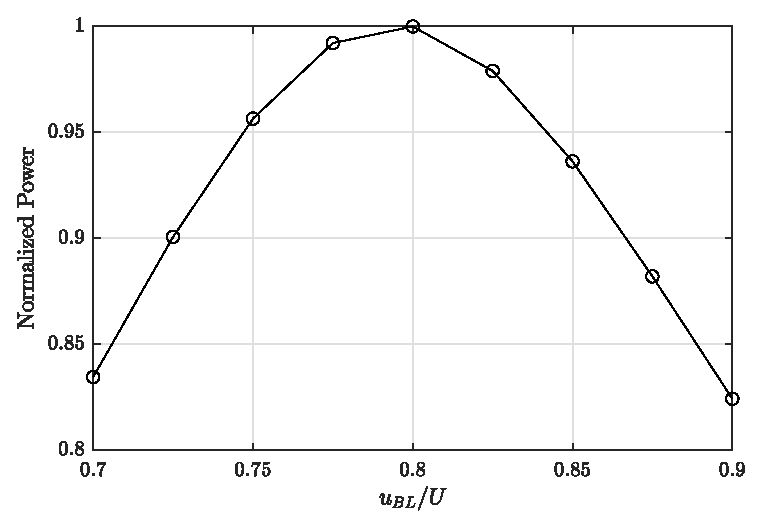
\includegraphics{../matlab/06_single_sensor_filtering/filter_velocity_measure.eps}
 \caption{Boundary layer velocity measurement of the synthetic wavefront using a combination of a low-pass velocity filter and a high-pass radial frequency filter. The maximum value at $u_{BL}/U=0.8$ corresponds with the actual value used in the creation of the synthetic wavefront.}
 \label{fig:06_filter_velocity_measure}
\end{figure}
The low-pass velocity filter used the same parameters as used previously except that $u_x$ was varied and the high-pass radial frequency filter used a cutoff value of 0.1 with an order of $n=2$.
The radial frequency, $\xi_\rho$, was normalized by the spatial sampling rate.
In this case, the boundary layer speed was determined to be 163 m/s which corresponds to the design velocity of the synthetic signal of $0.8U$.
For signals where the mean-velocity component of the aero-optical signal is not aligned with either the horizontal or vertical axis, both velocity components can be varied in the velocity filter.
This produces a three-dimensional surface of filtered signal power as a function of $u_x$ and $u_y$ in the velocity filter, where the velocity components of the moving signal are given by the maximum power of the surface.
An example of this method is shown in Figure \ref{fig:06_filter_velocity_real}, which was computed using experimental wavefront data acquired in the White Field wind tunnel at M=0.5.
\begin{figure}
 \centering
 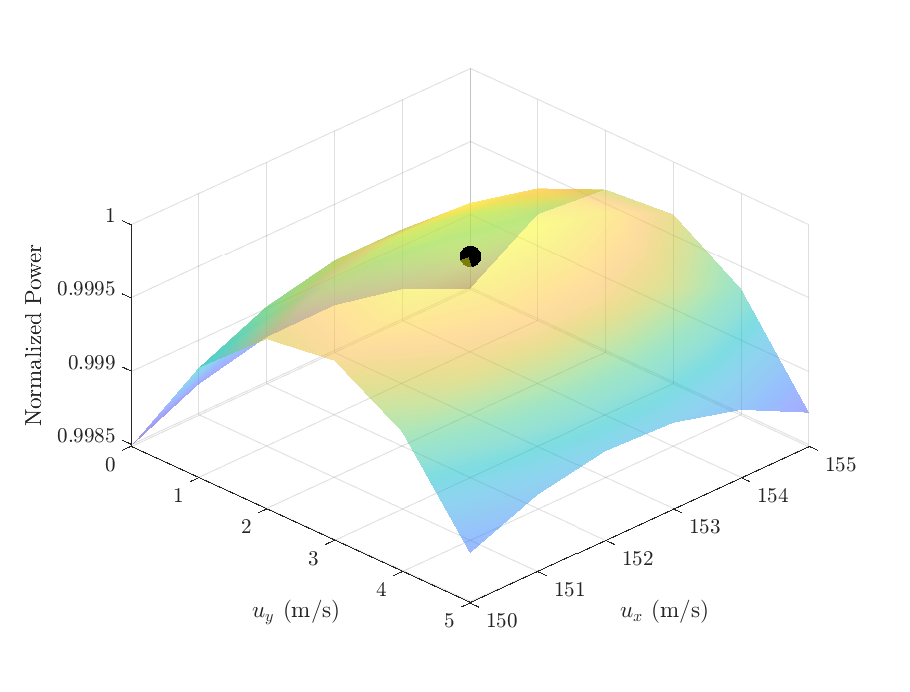
\includegraphics{../matlab/06_single_sensor_filtering/filter_velocity_real.eps}
 \caption{Velocity low-pass filter used to determine the mean disturbance velocity of measured data presented in Figure \ref{fig:04_dispersion_3d}.  The velocity in the x-direction was measured to be 152 m/s and 3 m/s in the y-direction.}
 \label{fig:06_filter_velocity_real}
\end{figure}
In this case the same filtering parameters were used as the synthetic case except the distance cutoff was $d_c=1/40$ and both $u_x$ and $u_y$ were variables.
The velocity components of the boundary-layer optical disturbances determined from Figure \ref{fig:06_filter_velocity_real} are 152 m/s in the x-direction and 3 m/s in the y-direction.
This boundary-layer velocity is approximately  times the freestream velocity when compared to the pitot probe measurement of the free-stream velocity, which is very close to the accepted speed of the optically-aberrating structures in a boundary-layer flow.
The overall flow angle of the boundary-layer with respect to the orientation of the measurement beam was approximately $1.1^\circ$.

\section{Baseline Spectrum}
\label{chap:06_baseline}
If all of the narrow-band temporal signals in a data set can be assumed to be measurement contamination that needs to be filtered out, a method for calculating the baseline of the spectrum would provide a simple way of filtering a portion of the signal contamination.
For example, during analysis of Raman spectra, the baseline spectra must often be removed \cite{Schulze-2012-GmyAqzC7}.
This task is often performed manually which has resulted in a number of attempts to create automated techniques to estimate the baseline spectra \cite{Mosier-Boss-1995-keK3ckUN, Schulze-2005-QkUeywxD, Schulze-2012-GmyAqzC7, Zhao-2007-HAc6j8Wb}.
One of those techniques \cite{Schulze-2012-GmyAqzC7}, a small-window moving-average based, fully automated baseline estimation method was used in this research.
For this method, at each spatial frequency location, the baseline spectrum was computed along the temporal axis.
This process estimates the baseline spectrum, $\mathbf{b}$, from the measured spectrum, $\mathbf{m}$,
\begin{equation}
  \mathbf{m} = (\mathbf{b}+\mathbf{x})*\mathbf{p}+\mathbf{n} = \mathbf{b}*\mathbf{p}+\mathbf{x}*\mathbf{p}+\mathbf{n} \textrm{,}
\end{equation}
where $\mathbf{x}$ is a pure or underlying signal vector, $\mathbf{p}$ is an instrumental blurring function, $\mathbf{n}$ is measurement noise, and $*$ is convolution operator.

Figure \ref{fig:06_filter_baseline}, shows the multidimensional spectrum of an unfiltered measurement (top left) and its estimated baseline spectrum (top right).
\begin{figure}
  \centering
  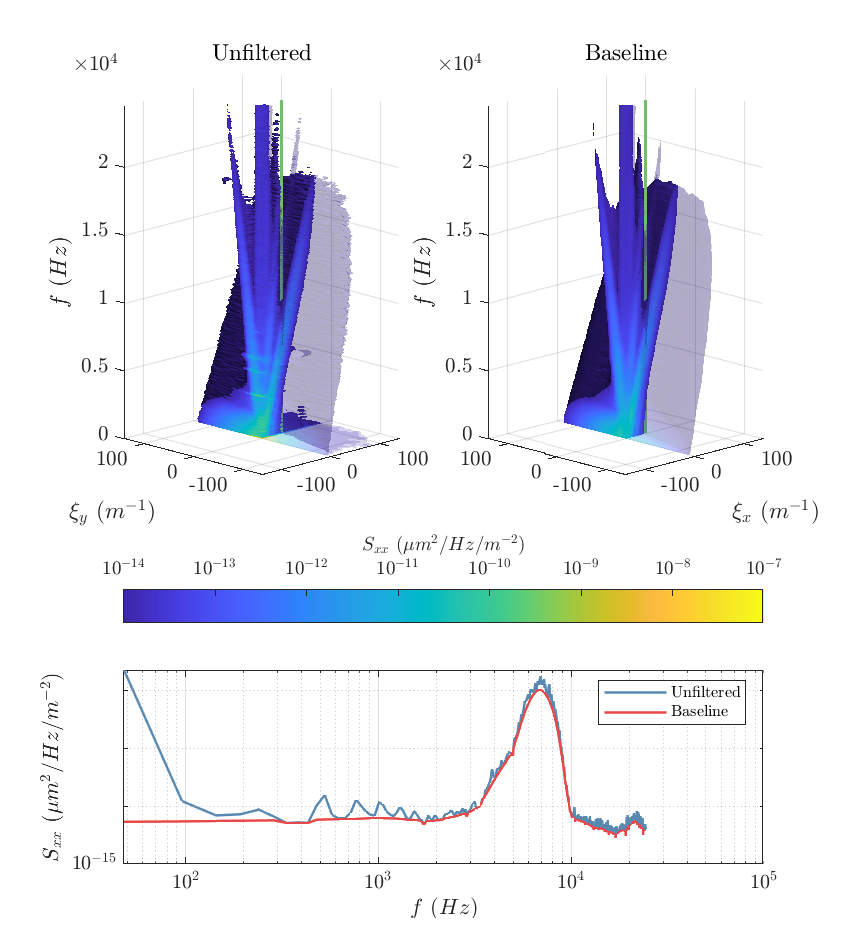
\includegraphics{../matlab/06_single_sensor_filtering/filter_baseline.eps}
  \caption{Baseline spectrum estimation. The top left plot shows the unfiltered multidimensional spectrum and the baseline spectrum on the top right. The green line in each of these plots represents the location at which the spectra in the bottom plot is shown.}
  \label{fig:06_filter_baseline}
\end{figure}
The bottom plot of the figure shows the unfiltered and baseline spectra along the green line in the two multidimensional spectral plots.
The total power of the signal has been reduced by $~71\%$ with all of the narrow-band signals removed.
A large portion of this signal removal is the very low temporal frequency components.
The blade-passing frequency and harmonics are completely removed but the broadband acoustic duct-modes remain intact.
The peak of the boundary-layer signal is reduced slightly as well as the high frequency fluctuations.

\section{Basic Filter Summary}
Three different basic wavefront filters were shown and discussed in this chapter.
The temporal filter is most useful when filtering out a frequency band of optical noise.
Besides filtering out optical noise, band-pass filters can be used to analyze a wavefront over a narrow-band to examine the optical aberrations at specific frequencies that significantly contribute to the overall optical disturbance; for example, as was shown in Chapter \ref{chap:03_optical_acoustics}, band-pass filters along with an implementation of an acoustic mode-marching method can help determine with some confidence that a narrow-band signal is likely to have been created by the wind-tunnel fan and can be removed.

Filters that separate upstream and downstream-moving disturbances are useful to filter out the optical contamination that comes from acoustic signals that are traveling upstream from a wind-tunnel fan.
These filters would also be useful for separating out an aero-optical signal that has a broad range of velocities that can occur in a span wise measurement of a boundary layer.
The velocity filter is the most useful for isolating the aero-optical portion of a wavefront measurement given the aero-optical signal has a fairly narrow and constant velocity range.
This filter also can be used to measure the speed associated with an optical disturbance in both x and y-directions.

The spectral baseline provides an simple way of removing all of the narrow-band signals with slight attenuation to the broadband signals.
The broadband acoustic and stationary modes remain but could be filtered with via other techniques such as using a velocity filter.
Narrow-band features that are not likely to be environmental contamination could be easily added back in.
